\appendix
\section{Detailed Methods Section}

\begin{figure*}
    \centering
    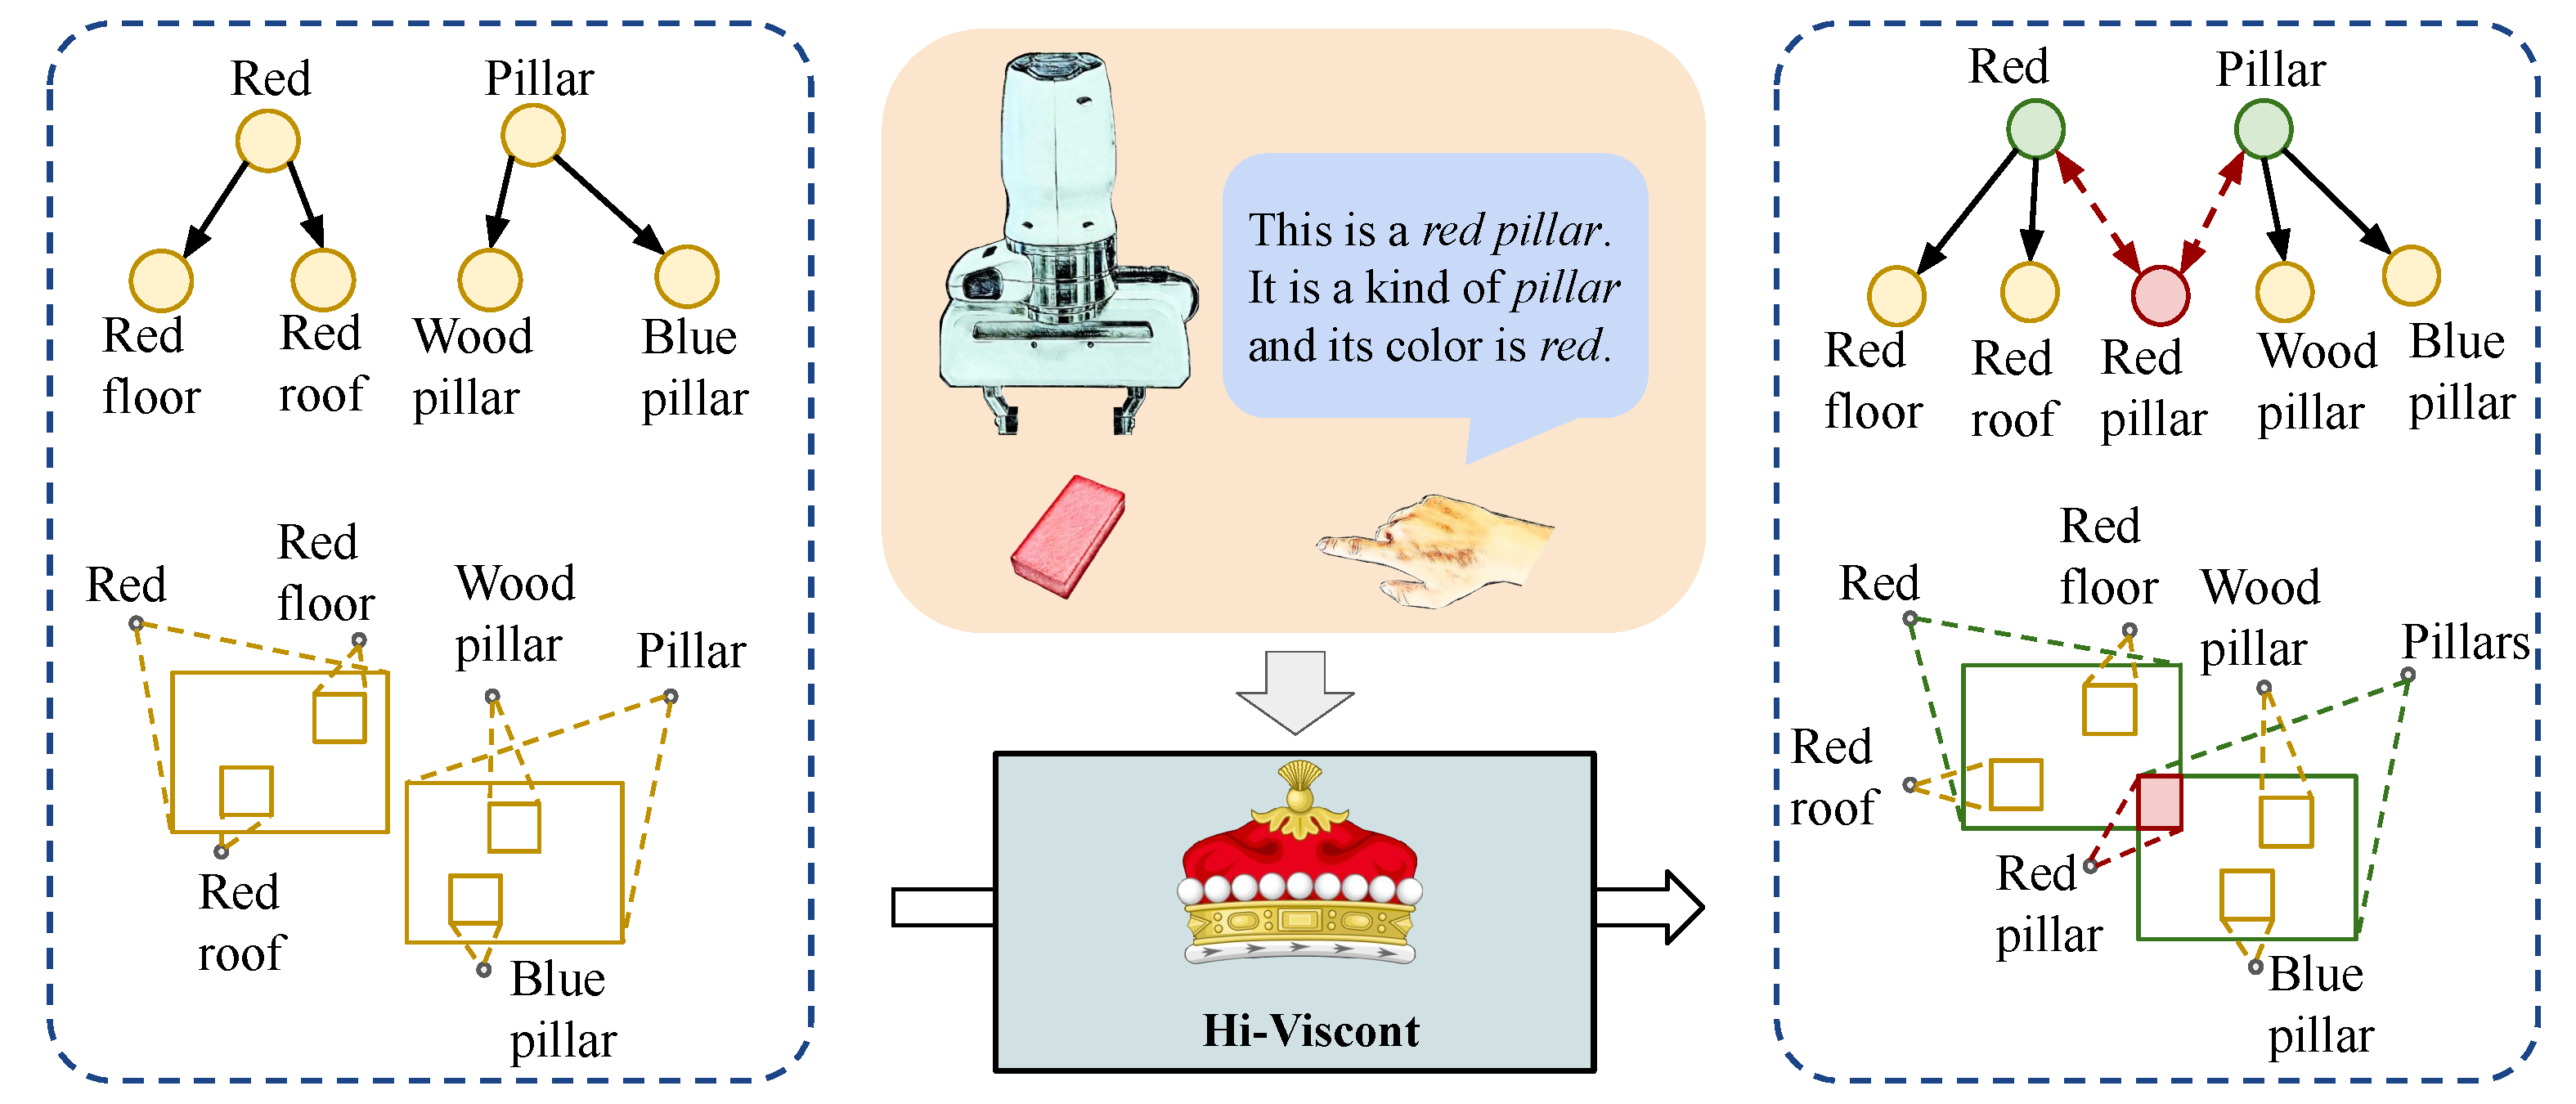
\includegraphics[width=0.8\textwidth]{figures/figure2.pdf}
    \caption{We demonstrate the updates to the box embedding space and the parent concepts when a novel concept is taught to our robot using Hi-Viscont. Existing approaches only edit the leaf nodes as those represent novel concepts.}
    \label{fig:concept_net_model}
    \vspace{-5mm}
\end{figure*}

% introduce FALCON
% With more details, this should take about 3/4 of a column
We first present the baseline FALCON model and then introduce our Hi-Viscont model. We based our model on concept learners as they can be taught concepts few shot, and they can reason over the attributes of chosen (and their parent) concept classes. FALCON is the SOTA concept learner which learns novel concepts one-shot. 
% Details for why FALCON
% The ability of learning concepts on the fly is necessary for robots to perform tasks because robots will run into unknown objects or concepts when they are performing the task, and such ability can quickly adapt robots to unseen tasks.
% Therefore, we hope to adopt one-shot learning framework to the robotic domain.


\subsection{FALCON}
% The task that FALCON solves
%   One-shot visual concept learning
%   Answer visual reasoning questions
\citet{mei2022falcon} developed FALCON, a meta-learning framework for one-shot concept learning in visual domains.
FALCON learns a new visual concept with one or a few examples, and uses the learned concept to answer visual reasoning questions on unseen images.
There are three components for the FALCON model: a visual feature extractor that extracts the object-centric features for the input image, a graph neural network (GNN) based concept learner, and a neuro-symbolic program executor that executes the input neuro-symbolic program.
% go through a bit the neuro-symbolic programs
The neuro-symbolic programs are structured representations constructed from natural language sentences.
FALCON learns novel concepts by interpreting the images presented and the relationships between known concepts and the unknown concept being learned given a neuro-symbolic program. 
After learning FALCON performs reasoning over questions, executed as neuro-symbolic programs to answer questions about images. 
% By executing these neuro-symbolic programs, FALCON learns novel concept by interpreting the image and the relations with other known concepts, and performs reasoning on visual reasoning questions.
% FALCON's visual feature extractor
FALCON uses a pre-trained ResNet-34 as visual feature extractor.
The input to the visual feature extractor is the mask for each object of the image and the original image.
The visual feature extractor computes an embedding vector for each of these objects, which will be used for downstream visual reasoning.
% Box embedding
FALCON uses the box embedding\citep{vilnis2018probabilistic} as representations for concepts and the object-centric visual features.
%In the box embedding space, a concept is represented as a high dimension box. The embedding of a concept is a tuple of two vectors: $e_c = (\text{Cen}(e_c), \text{Off}(e_c))$, denoting the center and the offset of the box embedding.
% GNN
The concept learning module of FALCON is composed of two separate Graph Neural Networks(GNNs), the relational GNN and the example GNN.
To predict a embedding for a novel concept $c$, FALCON first samples random prior embedding as the representation for $c$ from a Dirichlet distribution.
Then, FALCON updates the embedding of $c$ by computing a message from the related parent concepts to the novel concept based on their relationships using the relational GNN.
FALCON further updates the representation of $c$ by computing the message from the visual feature of the object that serves as the example of the novel concept to the embedding computed by the relational GNN. The resulted representations are the candidates for the representation of the novel concept $c$.
FALCON then uses the candidate representation that has the highest data likelihood as the representation of the novel concept $c$, denoted $e_c = e_c^k; k = argmax_i P(e_c^i\mid o^{(c)})$, where $o^{(c)}$ is the visual representation extracted from the train image, $e_c^i$ is the candidate embedding for concept $c$, and $e_c$ is the final representation for concept $c$.
\citealt{mei2022falcon} trained the concept learning module by using the computed representation of the novel concept $c$ for visual question answering task.

%The concept learning module takes the relations between the novel concept and other known concepts, and the visual features of the object that serves as the instance of the novel concept as inputs. 
%Each relation with a known concept $c'$ is a 3-tuple $(c, c', rel)$, where $rel$ denotes the relationship of $c$ with $c'$. We denote the collection of these relations as $R_c$.
%Because the representation for the objects in the example image is also in the same embedding space, FALCON treats them as another related concept to the novel concept $c$ with a special relationship $r_o$. We denote the representation of these objects as $o_c$

%These priors are treated as the initial embedding for the novel concept $c$.
%$GNN_1$, also known as the relational GNN, updates the embedding for concept $c$ by computing a message from the relations $R_c$ to the initial embeddings $e_0^i$. We denote this as $GNN_1(R_c, e_c^{0,i})=e_c^{1,i}$. 
%$GNN_2$, the example GNN, treats the features of the example object of the novel concept $c$ as a related concept to $c$, with a unique relationship. 
%The example GNN then updates the embedding for $c$ by computing the message from the features of the example messages to $e_c^{1, i}$, this process is denoted as $GNN_2()$
 

% Why FALCON is insufficient?
Although FALCON introduces the powerful idea of learning visual concepts on the fly, it remains insufficient for interactive visual task learning for two major reasons.
%   1. FALCON does not learn the task
Firstly, the FALCON model is not designed for task learning. Even though the model is able to recognize the objects that are used for the visual tasks, it does not know how to pick or place the objects.
%   2. FALCON assumes that its knowledge of concept is perfect
Secondly, FALCON is designed with an assumption that the model has a perfect knowledge of its known concepts, and hence once a concept is learned, its representation will never get updated as the model learns more concepts.
% Such assumption may not be true under the real world scenario, and the flaw of such design gets more obvious when we have less or no prior knowledge about the concepts.
For example, when we teach the model the concept of "container" with an image of a cup, the FALCON model registers the embedding for the "container" concept using the features of the cup including its handle. 
Later, when we teach the model about the concept of a "bowl", we can describe to the model that the "bowl" is a "container". However, FALCON cannot update the embedding of "container" with the newly added knowledge and feature information.
% , and hence fail to recognize an image of a bowl as a container, even though we explicitly told the model about this information. 
% Therefore, such assumption needs to be removed for a robot to actively update its knowledge about the world, and utilize those knowledge to perform variants of tasks. 

\subsection{Hi-Viscont}
We present our concept net model, Hi-Viscont, which actively updates the related known concepts when we introduce the novel concept.
% introduce which part we adopted from FALCON
We adopted several modules from the framework of FALCON, including the visual feature extractor, the neuro-symbolic program executor, the box embedding space, and the novel concept learner.
% That is to say, our concept net model learns the representation of the novel concept in the exact same way as FALCON.
% introduce the new gnn
However, we introduce an additional module that updates the related known concepts when a novel concept is introduced. 
We use an additional GNN, namely $GNN_3$, to predict a new embedding for the related known concepts, by computing a message from the visual feature of object of the novel concept to the embedding of the related nodes using the relations between the related concepts and the novel concept.
\wgnote{Describe GNN 3}
When a novel concept $c$ is inserted to Hi-Viscont, the extracted visual feature $o_c$ of concept $c$ and its relations with known concepts $R_c$ are fed to Hi-Viscont as input. 
Each relation $rel=(c',c, r)$, where $c'$ denotes the related concept, and $r$ describes its relationship with $c$.
Using $GNN$




To provide gradient flow to train $GNN_3$, we extended the concept learning task proposed by FALCON by adding validation questions for each related concept. That is, during training, when a novel concept $c$ is inserted, we will update the embedding for all the related concepts(including $c$), and we will use all of these embedding for visual reasoning task, to jointly learn to predict the representation of the new concept and update the representation for the known concepts.
%We describe how our algorithm update the embedding of the concepts as follows:
%\begin{algorithm}
%\caption{Concept Learning Algorithm}
%\begin{algorithmic}[1]
%  \scriptsize
%  \STATE \textbf{function}: Insert-Concept($c$, $R_c$, $o_c$)
%  \STATE    Sample prior embedding from Dirichlet distribution: $e_c^{i,0}\sim p_{D}$
%  \STATE    Update embedding by computing message from related known concepts to the prior embedding: $GNN_1(e_c^{i,0}, R_c) = $
%\end{algorithmic}
%\end{algorithm}
% Describe our training algorithm
We also developed a new training protocol to train our concept net model.
The concepts from the dataset is divided into three groups: $C_{pretrain}, C_{train}$ and $C_{test}$, where the pre-train concepts $C_{pretrain}$ represent the pre-existing nodes in the knowledge graph.

The training of the concept net model is consists of three stages, the pre-training for the visual feature extractor, the pre-training for the embedding of pre-train concepts $C_{pretrain}$, and the training to update the knowledge graph with train concepts $C_{train}$.
The details for the pre-training protocols can be found in the appendix.

After we have pre-trained the visual feature extractor and the embedding for the pre-train concepts,  we train the concept learner module during the training stage. 
We freeze the weights of the visual feature extractor at this stage because otherwise the embeddings for the pre-train concept will not be usable. 
Because we hope to train $GNN_3$ to update the embedding for known concepts with information from unseen instances, we have to reset the embedding for all the train concepts $C_{train}$ after all the train concepts are inserted to the network.
%The resetting mechanism also reduces the issue brought by the bad embedding predicted by the initial weight of the module, because the model will see the meaningful embedding again after a certain period. Empirically, after certain iterations of training, our $GNN_3$ can update the known concepts with meaningful embedding.
After inserting all the concepts within the train set in the final round, we do not reset the embedding for the train concepts and insert the concepts in the test set $C_{test}$. 
While FALCON is evaluated solely on the newly inserted concept, we evaluate all concepts of our model on unseen images. This ensure consistency parent and child concepts which is a necessity in continual learning settings. 
This evaluation mechanism allows us to evaluate the quality for the embedding of all concepts in the resulted knowledge graph, which is closer to how these knowledge are used in the real world setting. 




% introduce our concept net model
%The concept net model maintains an extensible knowledge base of concepts, and it uses the concepts that it knows to perform reasoning and answer visual questions.
% How the model is trained
% Trained with augmented concept learning task
%We trained our concept net model to learn visual concepts in one-shot using the concept learning task.
% Define the concept learning task
% We should start from the programs here, because FALCON says that t
%We formulate the concept learning task as a 5-tuple: $(P_t, I_t, P_r, P_v, I_v)$, where $P_t, P_r$ and $P_v$ are neural-symbolic programs parsed from the sentence that described the novel concept, the sentence that describes the relations of the novel concept with other concepts, and the visual reasoning questions respectively.
%The other inputs $I_t, I_v$ are images along with object-centric bounding boxes also provided by the upstream models.
%Different from FALCON, our validation questions will involve not only the novel concept, but also all the related known concepts. 
%This allows our concept net model to also update the embedding of known concepts with newly introduced information, and thus remove the assumption of FALCON that the model knows the known concepts perfectly.
%We also use the box embedding space \cite{vilnis2018probabilistic} as representation for both the concepts and the object-centric visual features in our concept net model, because it fits well in the context of learning a hierarchy of concepts.

% describe the architecture that learns concept in one-shot
% 1. visual feature extraction
%When we try to teach the robot a novel concept $c$, we first extract the object-centric visual features from $I_t$ and $I_v$ using a pre-trained ResNet-34\cite{he2015deep}, denoted $e_t = $ ResNET $(I_t)$ and $e_v = $ ResNET $(I_v)$.
% 2. embedding prediction module
%To predict the embeddings for $c$ and update the related known concepts $\{c_1,\dots, c_m\}$, we feed the extracted visual features of the train image $e_t$, the train neural-symbolic program $P_t$ that describe the concept in the train image, and the neural-symbolic program $P_r$ that describes the relations with the related concepts into our embedding prediction module.
%We use three graph neural networks (GNNs) with different weights to predict embeddings, which we denote $GNN_1, GNN_2,$ and $GNN_3$ respectively.
% introduce how we compute the embedding of the novel concept
% notations for embeddings might not be good, how 
%$GNN_1$ and $GNN_2$ are used to predict the box embedding for the novel concept $c$, while $GNN_3$ is used to update the known related concepts $\{c_1,\dots, c_m\}$.
%We first randomly sample multiple priors $e^{i,0}_c$ from a Dirichlet distribution as the initial representation of the novel concept $c$.
%We first compute the message from the related known concepts $\{c_1, \dots, c_m\}$ to the novel concept $c$ based on their relations with $c$. We denote such relations as $RELS = \{rel_1, \dots, rel_m\}$.
%Each relation $rel_i$ is a tuple of the known concept and the relation type $(c_i, r_i)$.
% GNN_1 computes message from parents to concept c.
%By executing $P_r$, $GNN_1$ will update the prior embedding with the relations $RELS$, denoted $GNN_1(e_{ci}, r_i, e^{j,0}_c) = e^{j,1}_c$.
% GNN_2 computes messages from concept instance to concept
%Then, we use $GNN_2$ to compute the updated information brought by the example objects' visual feature $e_t$. We treat $e_t$ as a related concept, which has a unique fixed type of relation $r_t$ with the novel concept $c$. By executing the train program $P_t$, $GNN_2$ updates the for the novel concept $c$, denoted as follows: $GNN_2(e_t, r_t, e^{j, 1}_c) = e^{j,2}_c$.
%We then choose the embedding for the novel concept $c$ among the embeddings generated by different priors by picking the one that entails the $e_t$ most, denoted $e_c = e_c^{k, 2}; k=argmax_{l}P(e_c^{l,2}|e_t)$.
% GNN_3 computes messages from instance of novel concept to related concepts
%Additionally, we use $GNN_3$ to compute a update message from the visual features of the instance of the novel concept $c$ to the related concepts based on the same relations $RELS$. We denote this as $GNN_3(e_t, r_i, e_{ci}) = e_{ci}'$. 
%We then use the embedding of the novel concept $c$ and the updated embedding for the related known concepts $e_{ci}$.


\subsection{Learning Visual Task via Scene Graph}
To learn a visual task from a single in-situ interaction with human user, we first convert the user's demonstration into an initial scene graph.
Each node of the initial scene graph correspond to one object that the user placed, and it contains the bounding box information of the object and the user's linguistic description of the object.
For each node of the initial scene graph, we also store its positional relations with other nodes, which are computed with the bounding box information.
These positional information will be used to compute the placement location of objects when later the robot attempts to reconstruct the scene.
We mark a fixed location with black tape on the table, which serve as the origin and is treated as the first object. All other objects placed by the user will be to the top right of the origin, and the location of the origin is always known to the robot.
The other nodes will be sorted as an ascending order from bottom to top and from left to right.
%In this work, the positional representations only contain information of directions. 
%When looking for the placement location of an object, we only refer to the relation with its nearest neighbor, and we will place the object in the direction denoted in the relations with a fixed distance. 
%
Then, based on the initial scene graph and the user's linguistic request for the variant of the visual task, we infer a goal scene graph which provides the robot information about the object to pick and location to place.
Since the variant of the visual task from the user request share the same structure as the demonstration, the goal scene graph is to have the same number of nodes as the initial scene graph, and the positional relations between each pair of nodes remain the same.
Therefore, we directly copy those information for each node from the initial scene graph. 
By doing this, we have simplified the inference of the whole graph to the inference of object information of each node.
%Notice that in this work we do not directly copy the bounding box information from the initial scene graph for a direct access to the placement location, this is because that the variants of object size in each location.
We take the the user's description of the corresponding node of the initial scene graph $t_i$ and the user's linguistic request of the variant of the structure $q$ as inputs, and perform a 2-step inference.
Firstly, we perform a binary classification for each node to decide whether the related concepts in the scene change given the user's description of the node and the user's request $q$. 
We use a pretrained BERT\textsubscript{base} model to encode the context request pair in the format of \\
$$[CLS] context [SEP] request [SEP]$$
The embedding of the $[CLS]$ token is treated as the representation for sequence, and is fed into a MLP classifier for the binary classification.
The second step of the inference extracts the related concepts from the context.
We convert the concept extraction problem into a classification problem by providing concept candidates as a part of the input.
The input to the concept extraction model will be a natural language sentence $s$ and a list of candidate concepts $\{c_i, 1\leq i \leq m\}$.
We concatenate the natural language sentence with each of the concept candidate respectively using the format of 
$$[CLS] s [SEP] c_i [SEP]$$
We then feed the $[CLS]$ tokens of these sequences to a MLP scorer to get a score for each concept candidate conditioned on the natural language sentence. 
The normalized scores are treated as the probability distribution over the concept candidates.
The context and the concept candidates can be different depending on the use case and the classification result of the previous stage.
As a result, each node of the goal scene graph now contains information of related concepts and positional relations with other nodes.
The related concepts of each node is fed as input for the concept net model to decide the object to pick, and the positional relations with other nodes are used to compute the placement location.
The robot will reconstruct the scene following the order of the nodes.
For each node, the robot picks the object according to the concept net model.
The placement location of each object is at a fixed distance to the direction indicated by the relation with its closest neighbor that is placed.
Pairing the concept net model with scene graph, the robot is able to learn the placement of a scene in one single demonstration and perform variants of the scene without demonstration.



\subsection{Robotics Setup for User Study}
We integrate our visual task learning and concept I build thelearning model with a Franka Emika Resarch 3 arm(FR3). 
% Our complete pipeline learns a new object conceptually with the help of its visual features and a description, get a user query to create a new scene, recreate a scene learned from the scene graph learned from the user demonstration with the change mentioned in the query.
This pipeline allows us to show the generalizability with which Hi-Viscont learns visual concepts when compared to Falcon \ngnote{Falcon's citation} in learning and solving novel tasks. 
To set this demonstration up we use a Franka Emika Research 3 arm (FR3), two calibrated realsene D435 depth cameras, and a mono-colored table. 
It is important to use a mono-colored table for us as we use SAM(Segment Anything Model) \ngnote{use Sam citation} to separate the foreground and the background and get individual bounding boxes for each of the blocks on the table.
Initially, we looked into Google's Transformer net \ngnote{citation of transformer network}. 
% We aimed to create a simple scene-building mechanism that is able to pick objects based on the classification from the place camera frame and rebuild a scene in the scene place in the place camera frame.
but used a simpler Visual Motor Servoing mechanism for reliability.
% The pick scene camera requires calibrating the pick scene camera with respect to the FR3 base frame. 
% We take multiple pictures in different configurations of the FR3 end-effector to which an acuro market is attached. This allows us to find a Transformation Matrix which converts the coordinates from the  camera frame  to the Robot  base frame. The place scene camera is used to find the length of the object occupying the current node of the scene graph. 

SAM is used to segment the objects placed in the place scene and find the bounding boxes of each placed object which are also the nodes of our scene graph.
% This allows us to calculate the position of the next object by finding the relative position of the next node with respect to the current object being placed.
% , referencing the position of the node of the scene, and calculating the length of the bounding box of the referenced node. 
% we use a formula of shift = 1/2*max(bounding box of the referenced node length)+50 pixel space \textbf{Next node position}= Relation to the reference node(Reference node position,shift). The function relation to the reference node adds a shift to the reference node position based on its relation to the next node. For example, it adds the shift only to the x coordinate if there is "to the top of" relation, or in the case of "to the right of" relation, it adds only the y coordinate of the current position. In our scene graph, we are able to identify "to the top of ", "to the bottom of"," to the right of"," to the left of", "to the top right of"," to the top left of"," to the bottom right of", and "to the bottom left of" relations.\\
% The Segment Anything Model is capable of separating the foreground from the background. This allows us to find the table mask and the segment of each object placed in the camera frame on the table. \\
The flow of our pipeline requires us to first demonstrate the visual scene with all the objects placed in the Task scene to make a structure with linguistic inputs. 
We have to make sure that the objects are placed at a distance that allows SAM to create separate segment boxes for the objects. Then we pass each segmented object to either FALCON or Hi-Viscont classifiers to classify conditioned on the given language query. The robot then picks the object with simple visuo-motor servoing. 
% by the node information of the scene graph. 
% Once we find the object to be picked we then calculate the center of the bounding box of that object and convert it to the Robot frame with the help of the transformation matrix. 
If in the process there is an incomplete or erroneous grasp, we reattempt the whole classification again autonomously. Once the object is grasped we then place the object into the Task scene, with the position calculated relatively with respect to the previously placed object node or \ngnote{the ground object??}. This process is iteratively done until we have completed the whole scene graph.

\subsection{Human-Subjects Experiment}
\subsubsection{Study Design}
We conducted a 1 $\times$ 2 within-subject experiment to measure the framework's ability to learn visual task and visual concepts from in-situ interaction.
We extended the FALCON model with our scene graph module and use it as a baseline to compare against because we could not find any prior work that enable robot to learn a task from in-situ interaction.
We trained both concept net models with the same split of concepts and the same training data for the same number of steps.
Through this experiment, we demonstrate that our framework achieves better performance than FALCON model because of the continual update for the known knowledge.
Participants for our experiment interact with the robot in three phases.
For each interactive phase, the participants only interact with the robot once, and the interaction is recorded as the input for both systems.
After the interactive phases, the participant observes the two systems construct the scene requested by the participant. We keep the initial conditions the same for both systems. The participants observe both systems construct the scene with randomization in the order in which they observe the FALCON or our Hi-Viscont system first.   
% To remove the confounding factor, the participants are into two groups equally, and each group observes the reconstruction of the two systems in different order.
\subsubsection{Domain}
We evaluate our approach with the human-subjects experiment in a 2D object rearrangement domain, which is a problem that is commonly used in language grounding and HRI research~\citep{liu2021structformer, shridhar2021cliport}.
The domain we choose for this the House-Construction domain introduce in Domains Section.
We used a building blocks from children's toys as they are easy to grasp and grasping is not the focus of this work.

\subsubsection{Metrics}
The objective metrics we collect for the human-subjects experiment are as follows. 
We measure the success rate (SR) of completing the user's request, and the node level accuracy of each scene graph for both systems.
Both metrics are used to measure each system's ability to actually complete the visual task objectively.
The success rate gives us the insight of system's ability of completing the whole task, while the node level accuracy provides a more fine-grained idea on how accurate the system is doing in object recognition.

\ngnote{Do subjective tests and cite them here!}
% The subjective metrics we collect for the human-subjects experiment are as follows(the details of hand-crafted surveys, Cronbach's alpha, qualitative results, and quotes from interview questions are in the Appendix).
In the post-study survey for each system, we administer the Perceived Intelligence and Likeability sub-scales of the Godspeed Questionnaire Series\cite{Bartneck2009MeasurementIF}.
We additionally ask participants seventeen post-study questions.
In addition, we hand-crafted a comparison survey, which includes eight questions in the comparison survey for a direct comparison between our framework and FALCON model.

\subsubsection{Procedure}
This study is approved by our university's Institutional Review Board (IRB). We recruited all participants through on campus advertisements. 
The study took $90$ minutes. The participation was voluntary and the participants were not compensated for their efforts. 
The procedure of the study is as follows. 
Participants first fill out the pre-study survey.
After the pre-study survey, we hand out a general introduction for the experiment of the study.
Then, we guide the participant through the task teaching phase, the concept teaching phase, and the request phase sequentially. 
% We will discuss about the tasks for each of these phases below.
Before each phase, we provide a demonstration video and the manual of the corresponding phase to the participants. The domain used in the instruction videos is demonstrating a different task (bridge making) with different objects (foam blocks) than the actual task the participant is teaching. 
The anonymized instruction manual and the link to these videos are provided in the Appendix.

\paragraph{Task Teaching Phase - } In the task teaching phase, the participants will teach the robot a visual task by demonstrating the scene with its constituent structures one by one. The participants also describe the structures and the objects used to build the structure with natural language. For example, a participant might build a house, with floors, pillars and a roof. While building the roof participant might say ``This a roof which I build with the curved blue tile because of it's sheltering capability.'' The participants will demonstrate each of the structures with their associated language command one after another to build a house. We record all descriptions in audio and convert them into text using audio to text tools.  
% which object they choose to build that node, and the reason for choosing such object. 

\paragraph{Concept Teaching Phase - } In the concept teaching phase, the participants teach a novel concept of their choice to both systems by showing the object to the camera, and describing the concept's properties such as the color of the object and the functional characteristics of the object, in natural language. 
The description to the novel object concept will be converted to neuro-symbolic programs. These neuro-symbolic programs, along with the image of the object, are provided to both model to compute the representation of novel concept and its properties. The process of the update for the FALCON model is described in the \textbf{FALCON} subsection, and the process of the update for our concept net model is described in \textbf{Hi-Viscont}.

\paragraph{Request Phase - } In the request phase, the participants are asked to provide a request in natural language for a novel scene that they did not demonstrate in the task teaching phase with the object taught in the concept teaching phase. The task requested still needs to be a house which is the same task type as they demonstrated previously, but a house that has never been shown to our system.
\\

After completing the three phases, the participant will watch the two systems construct the scene based on their request in real time with the robot in a randomized order. 
After each system finishes the construction, the participant will be asked to fill out a post-survey for that system.
Finally, after both systems finish the construction, the participants will fill out a comparative survey.


% The participants will be asked to check whether the text converted from their audio accurately represents what they meant to say, and the experimenter will make minimum change to the text only with participants' permission.
% Additionally, we restricted the region for the 2D scene to be one side of the table due to the limited region that the robot arm can reach. 
% As mentioned in the \textbf{Learning Visual Task via Scene Graph} section, we marked an origin with a black tape on the table as the frame of reference for the systems to compute the placement location of the first object.
\subsubsection{Hypothesis}
\paragraph{Hypothesis 1 - } Our framework will have a higher success rate in completing the user's request. We hypothesize that our framework will have a higher success rate than FALCON model because of its update to the related known concepts, which could be used in requests that point to the same object indirectly.
\paragraph{Hypothesis 2 - } Our framework will have a higher node level accuracy. We hypothesize that our framework will achieve a higher accuracy in the node level than the FALCON model because that our model can correctly predict the object in the nodes that point to the object indirectly, while FALCON model does not handle these cases.
\paragraph{Hypothesis 3 - } We hypothesize that our framework will achieve higher ratings on subjective metrics compared to the baseline because of its higher accuracy and competency in completing the requests. In the nodes where our framework makes mistake, the mistakenly chosen object still share the same color as the true object, which is not the case for our baseline model.






% Introduce our method in an overall fashion
% In the style of going through the modules in the order of data flow.
%We propose our novel framework to learn novel visual concepts and visual tasks via in-situ interactions with human users.
% Define visual task
% Better definition(?)
%We define visual task as relocating a list of objects into the designated location based on the user's demonstration and request.
% How we learn the visual tasks
%The proposed framework learns an instance of a visual task from one demonstration by converting the demonstration, the descriptions for the demonstration, and the natural language request from the human user into a scene graph.
% What is the scene graph used for
%The scene graph provides the information about the location of placement for each object and the context for downstream models to infer the correct object to pick.
%We use a parser model to convert the contexts from the scene graph into neuro-symbolic programs as input for the concept net model.
% Describe the parser model
%The parser model is also used to parse user's description of the novel concept into neuro-symbolic programs when the user wants to extend the knowledge of the framework with a novel concept.
% describe our concept net
%We use a concept net model to learn novel concepts and infer the object to pick with the input neuro-symbolic model from the upstream module.
% the parts adopted from FALCON
%For our concept net model, we adopted the module to learn novel concepts and the executor of the neuro-symbolic programs from FALCON.
% The parent update
%Additionally, we introduced a new module to update the representation of the known concepts that are related to the newly introduced concepts.
% Cap
%With the information from the scene graph and the object to pick, our proposed framework will be ale to learn different visual tasks with one in-situ demonstration and perform variants of its known visual tasks using the concepts it knows.

%\subsection{Obtaining Initial Scene Graph}
% Introduce how we convert the user's in-situ interaction into a scene graph
%We convert the user's in-situ interaction for the task demonstration into a scene graph.
% Define input
% I: Initial image shown by the user, this is parsed into the initial scene graph
% D: the context of each node of the initial scene graph
% q: request
%An in-situ demonstration of user is a 3-tuple of $(I, D, q)$. where $I$ is the image of the goal condition of the demonstration from the user, $D={t_1,\dots, t_n}$ is a set of natural language sentences that describe objects $o_1, \dots, o_n$ that appears in $I$, and $q$ is a request from the user that requires the robot to perform a variant of the demonstrated visual task.
% Describe the creation of the initial scene graph
%We used a pre-trained SAM (Segment-Anything-Model) \cite{kirillov2023segment} to segment $I$ and obtain bounding boxes for $o_0,\dots, o_n$.
% describe the origin
%Notice that $o_0$ is a fixed location marked by us as origin to compute placement location of other objects, and we will explain in more details how this is done.
%For the sake of clarity, we will represent the objects as $o_1$ through $o_n$, arranged in ascending order according to their Euclidean distance from $o_0$ within the pixel space.
%We then create an initial scene graph $G_{init} = (V_{init}, E_{init})$.
% Initial nodes of the scene graph
%Each node $v_i$ of the initial scene graph corresponds to an object $o_i$ from $I$ respectively, and contains the corresponding bounding box information and description in natural language $t_i$.
% Compute the edges
% The edges $E_{init} = \{(o_i, o_j, r)$ for $i, j\in \{0,\dots, n\}, i\neq j\}$ of the initial scene graph includes the positional relation between each pair of object. 
%Such relationships are computed using the positional information from each pair of nodes, which can be extracted from their respective bounding boxes.
% hard-coded distance
%In this work, the positional representations only contain information of directions. 
%When looking for the placement location of an object, we only refer to the relation with its nearest neighbor, and we will place the object in the direction denoted in the relations with a fixed distance. 
%This design is sufficient for our domain of human subject study, and this work does not revolve the problem of learning distances between objects.

%\weiwei{How to justify that the goal scene graph has the same number of nodes with the initial scene graph?}
%\subsection{Inferring Goal Scene Graph}
% introduce the goal scene graph and the parser model
%After obtaining the initial scene graph $G_{init}$ and the request $q$ from the user, we will infer the goal scene graph $G_{goal} = \{V_{goal}, E_{goal}\}$.
% The node of the goal scene graph contains a neural symbolic program for concept net
%Each node $v_i'$ of the goal scene graph contains the neural-symbolic program, which will be the input for the concept net model.
% assumptions: 
% 1: the goal scene graph has the same number of nodes and same positional relations between nodes
% Convert the inference for the whole graph into the inference of each node
%We assume that each node $v_i'$ of the goal scene graph corresponds to the node $v_i$ in the original scene graph, and the positional relations between nodes are the same as the initial scene graphs.
%Therefore, the inference of $G_{goal}$ is simplified into the inference of the nodes $V_{goal}$.
%To simplify the problem, we assume that the inference of each node $v_i'$ is independent from any other node $v_j'$. 
%We do the node level inference in two steps conditioned on the node context $t_i$ and the user's request $q$.
% Binary classification
%To infer for a node $v_i'$ of the goal scene graph, we first predict $P(o_i = o_i'\mid t_i, q_i)$ the probability that the object in the goal scene graph should be the same as the object of the original scene graph conditioned on the node context $t_i$ and the user request $q$.
%We use a pretrained BERT\textsubscript{base} model to encode the context request pair in the format of \\
%$$[CLS] context [SEP] request [SEP]$$.
%We then feed the embedding of the $[CLS]$ token as the representation for sequence into a MLP classifier for the binary classification.

% Introduce the parser
% Need some refinement, I am just dumping everything here RN
%Since we are using the downstream concept net model to infer which object to pick conditioned on a list of concepts, the structure of the output neural-symbolic program is static. 
%Therefore, the problem of parsing becomes extracting the list of concepts from the node context $t_i$ and the user's request $q$.
%We treat the extraction of concepts as a classification problem.
%The input to the model will be a natural language sentence and a list of candidate concepts.
%We concatenate the natural language sentence with each of the concept candidate respectively using the format of 
%$$[CLS] sentence [SEP] candidate [SEP]$$
%We then feed the $[CLS]$ tokens of these sequences to a MLP scorer to get a score for each concept candidate conditioned on the natural language sentence. 
%The normalized scores are treated as the probability distribution over the concept candidates.
%Depending on the inference from the binary classification, the input to the extraction is different.
%If the classifier decides that the node in the goal scene graph should have the same object as the node of the initial scene graph, we will feed the node context as the input sentence and the leaf nodes as concept candidates into the extraction model.
%On the other hand, if the classifier decides that the node in the goal scene graph is bound to change based on the request, we will do the following steps:
%We first try to directly extract leaf level concept from the request. If the extraction model predicts that no leaf level concept is mentioned, we try to extract a composition of non-leaf concepts from both the node context and the request.
%Because that the neural-symbolic program for one-shot inserting a new concept and the neural-symbolic program that describe the relations with other concepts also have a static structure, we use the same extractor to convert those inputs into neural-symbolic programs as inputs for the concept net model.
















% talk about the data flow of the framework
% user's demonstration -> scene-graph
%We first parse a user demonstration into a scene graph, of which nodes are contextualized with the description of the user.
% Information of each node: context and relations
% scene-graph with context -> concept in the concept net
%Our pipeline then infers the related concepts for each node of the scene graph based on the context, and feed the related concepts as inputs for our concept net model.
% detect object from the related concepts
%Conditioned on the input concepts and the input image, our concept net model picks the object with the highest probability among all possible objects in the image.
% Mention how to get the pick and place position

% Use SAM to get bounding boxes
%We used SAM(Segment Anything Model) to generate bounding boxes for objects.
%Using the bounding boxes, we can calibrate the robot with the camera to get the pick location for the robot.
%We infer the place location for each object based on the relationship with the grounded objects in the scene graph, which is also an object with a known location.

% Close it up with a summary of the pipeline





% Dataset Collection